\documentclass[11pt]{article}
\usepackage[margin=1in]{geometry}
\usepackage[T1]{fontenc}
\usepackage{lmodern}
\usepackage{microtype}
\usepackage{booktabs}
\usepackage{graphicx}
\usepackage{amsmath}
\usepackage{xcolor}
\usepackage{url}
\usepackage[hidelinks]{hyperref}
\usepackage[numbers,sort&compress]{natbib}
\usepackage{caption}
\usepackage{enumitem}
\setlist{itemsep=2pt,topsep=4pt}
\captionsetup{font=small,labelfont=bf}

\newcommand{\aqb}{\textsc{AQB}}

\title{\aqb: Can LLM Agents Do Release QA?\\[2pt]
\large A Benchmark of Planted Regressions in Real Android Apps}
\author{Anonymous authors}
\date{Draft, November 2026}

\begin{document}
\maketitle

\begin{abstract}
Coding agents now write much of the code in some software teams, and verifying that code is the
next bottleneck. We introduce \aqb{}, a benchmark that asks an LLM agent to do what a release QA
tester does: given a build of a real Android app and its release notes, find the regressions
before the release ships. \aqb{} contains 51 episodes over 9 open-source apps with 92 planted
regressions. Each regression is a real upstream bug, forward-ported onto a pinned head commit and
verified on a device against its fixed build. Agents drive an Android 15 device only through
screen tools, file structured bug reports and decide when to sign off; grading is deterministic,
with no model judge. We evaluate six agent configurations from three providers, each in its
vendor's own agent harness. The best agent catches 59\% of the regressions; the best strict pass
rate (every regression reported, then a sign-off) is 29\%; and 17 of the 91 observable regressions
(19\%) are caught by no configuration. The agent that catches the most bugs is not the one whose reports and
sign-offs are most trustworthy, and the ranking differs from a general intelligence index.
Agents reach almost every changed feature, but they do not carry out the verification steps
they are told to use: re-opening after a change, trying boundary inputs, and checking values
against what they should be.
\end{abstract}

% ---------------------------------------------------------------------------
\section{Introduction}

A ``software factory'' of coding agents can produce changes faster than people can test them. In
many teams the release gate is still a human tester who reads the release notes, exercises what
changed, and either signs off or files bugs. Two questions decide whether an agent can hold that
gate: \emph{does it catch the regressions that are actually there}, and \emph{can its reports and
sign-offs be trusted}?

Existing benchmarks do not answer them. Software-engineering benchmarks such as
SWE-bench~\cite{jimenez2024swebench} and Terminal-Bench~\cite{merrill2026terminalbench} measure
whether an agent can \emph{produce} a correct change. GUI-agent benchmarks such as
AndroidWorld~\cite{rawles2025androidworld}, AndroidLab~\cite{xu2024androidlab} and
OSWorld~\cite{xie2024osworld} measure whether an agent can \emph{complete a task} in an app that
works. Android testing benchmarks such as Themis~\cite{su2021themis} measure automated test
generators against real crash bugs, and LLM-based testers such as DroidAgent~\cite{yoon2024droidagent}
and VisionDroid~\cite{liu2025visiondroid} are evaluated on the bugs their own tool finds. None offers a
fixed set of planted regressions, with release notes and a release verdict, on which any agent's
findings can be compared.

\aqb{} is built for this question (Figure~\ref{fig:overview}). Each episode is a pre-release QA
sweep of one build that contains one to three planted regressions. The agent receives a short
brief with the areas to test, the seeded data, and a ``Changed in this build'' list written like
real release notes, which names every changed feature without stating a symptom or a trigger and
mixes in harmless changes. The agent tests the app on an Android device through screen tools,
files bug reports to a scripted developer, and signs off when it judges the build ready.

\paragraph{Contributions.}
\begin{itemize}
  \item A benchmark of 92 planted, device-verified regressions in 9 real Android apps, organised
    into 51 release-QA episodes with release notes and 93 decoy changelog lines (\S\ref{sec:bench}).
  \item A deterministic grading pipeline for free-text bug reports, anchored to what was on
    screen, with a blind-recall audit and a manual audit of rejected reports (\S\ref{sec:grading}).
  \item An evaluation of six agent configurations from three providers in their own harnesses
    (\S\ref{sec:results}).
  \item A behavioural analysis that splits every miss into ``ignored'', ``shallow'' and ``tested but
    not noticed'', and characterises the regressions no agent caught (\S\ref{sec:analysis}).
\end{itemize}

\begin{figure}[!t]
  \centering
  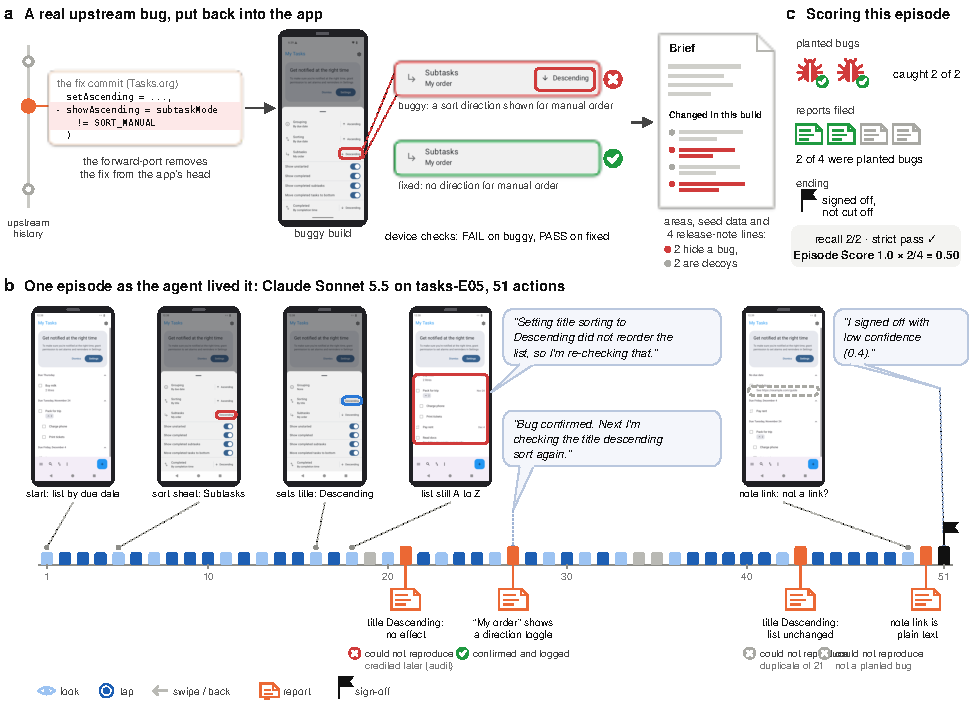
\includegraphics[width=\linewidth]{figures/p0_overview.pdf}
  \caption{\textbf{\aqb{} at a glance, with real artifacts from one episode.}
  \textbf{a}, A regression enters a build: the fix commit of an upstream bug in Tasks.org is
  reversed on the app's pinned head (red line). On a device, the buggy build shows a sort-direction
  toggle for a manually ordered list (red) where the fixed build shows none; the bug's checks fail
  on the buggy build and pass on the fixed one. The episode brief lists four changed features, two
  of which hide regressions (the colours are for the reader; the agent sees plain lines).
  \textbf{b}, The same episode as Claude Sonnet 5.5 lived it: the screenshots it requested (with
  the regressions it saw circled in red and its own action in blue), its own words, each of its 51
  actions by type, the four reports it filed and the scripted developer's replies, and the
  sign-off. One report was confirmed during the run; the report at step 21 was credited after the
  grader audit (\S\ref{sec:grading}); the report at step 50 described real but unplanted app
  behaviour. \textbf{c}, How this episode is scored.}
  \label{fig:overview}
\end{figure}

% ---------------------------------------------------------------------------
\section{Related work}

\paragraph{Agent benchmarks for software.}
SWE-bench~\cite{jimenez2024swebench} and its human-validated subset~\cite{openai2024sweverified}
grade code changes by running the repository's tests. Terminal-Bench~\cite{merrill2026terminalbench}
grades command-line tasks in containers. These benchmarks verify the agent's output with tests
written by people; in \aqb{} the agent is the tester.

\paragraph{Mobile and computer-use agents.}
AndroidWorld~\cite{rawles2025androidworld}, AndroidLab~\cite{xu2024androidlab} and
OSWorld~\cite{xie2024osworld} measure task completion in live environments with programmatic
success checks. Their apps are assumed correct. In \aqb{} the app is wrong in places the agent
must discover, and success depends on the agent's judgement, not on reaching a goal state.

\paragraph{Automated GUI testing.}
Random, model-based and search-based Android testers (DroidBot~\cite{li2017droidbot},
Stoat~\cite{su2017stoat}, Sapienz~\cite{mao2016sapienz}) and LLM-guided testers such as
GPTDroid~\cite{liu2024gptdroid} are usually evaluated on code coverage or crashes. Themis~\cite{su2021themis}
benchmarks such tools on 52 real crash bugs; Genie~\cite{su2021genie} targets non-crashing logic
bugs with an automatic oracle. DroidAgent~\cite{yoon2024droidagent} drives testing with an autonomous
LLM agent that sets its own testing goals, and VisionDroid~\cite{liu2025visiondroid} uses a multimodal
LLM to detect non-crash functional bugs, evaluated on 590 such bugs. These works propose a testing
tool and measure what it finds. \aqb{} instead holds the builds, the bugs and the grading fixed, so
that any agent can be compared on the same regressions, and it also scores the agent's release
verdict. Most \aqb{} regressions do not crash: they show a wrong value, lose a setting or ignore an
input, so catching them needs a judgement about intended behaviour.

\paragraph{Real-bug datasets.}
Like Defects4J~\cite{just2014defects4j}, \aqb{} builds each bug from a real upstream fix. Unlike
Defects4J, the bug is observed only through the app's screen, and the oracle is a set of device
checks rather than a test suite.

% ---------------------------------------------------------------------------
\section{The \aqb{} benchmark}\label{sec:bench}

\subsection{Apps}
\aqb{} uses 9 open-source Android apps (Table~\ref{tab:apps}). Four are mature projects with long
histories (Amaze File Manager, AnkiDroid, Markor, Tasks.org). Five are projects whose entire
history is from 2026 (Minus, Iris Gallery, Featherline, NerdCalci, Idle Fantasy). NerdCalci (a
notepad calculator) and Idle Fantasy (an idle role-playing game) are not form-and-list apps: most
of their bugs are plausible-looking wrong values that a tester must compute to catch. Every app
renders standard Android or Compose UI, so all visible text is in the accessibility tree.
Table~\ref{tab:apps} lists each app's upstream repository.

\begin{table}[!htbp]
\centering\small
\caption{Apps and the regressions planted in their episodes.}
\label{tab:apps}
\resizebox{\linewidth}{!}{%
\begin{tabular}{llllrr}
\toprule
App & Upstream repository (GitHub) & Licence & History & Episodes & Regressions \\
\midrule
Amaze File Manager & TeamAmaze/AmazeFileManager & GPL-3.0 & mature & 6 & 11 \\
AnkiDroid & ankidroid/Anki-Android & GPL-3.0 & mature & 8 & 15 \\
Markor & gsantner/markor & Apache-2.0 & mature & 6 & 13 \\
Tasks.org & tasks/tasks & GPL-3.0 & mature & 6 & 12 \\
Minus & isaacsa51/Minus & Apache-2.0 & 2026 & 6 & 8 \\
Iris Gallery & MohamadOday/iris-gallery & Apache-2.0 & 2026 & 3 & 3 \\
Featherline & mkx173/Featherline & GPL-3.0 & 2026 & 6 & 9 \\
NerdCalci & vishaltelangre/NerdCalci & GPL-3.0 & 2026 & 4 & 8 \\
Idle Fantasy & tristinbaker/IdleFantasy & GPL-3.0 & 2026 & 6 & 12 \\
\midrule
Total & & & & 51 & 92 (91 observable) \\
\bottomrule
\end{tabular}}
\end{table}

\subsection{Regressions}\label{sec:regressions}
\paragraph{Mining.} Each regression starts from a merged upstream fix: a commit or pull request
whose change corrects behaviour a user can see. We kept a fix when its bug (i) shows on the screen
or in data the app displays, (ii) is deterministic, and (iii) can be judged wrong by a tester
without access to the code; bugs whose only symptom is wording, or whose correct form a tester
cannot judge, were dropped. Of the 92 regressions in episodes, 52 come from mature projects and
40 from the 2026 projects; 58 were fixed upstream on or after 2026-01-01. Each is labelled with a
family (state 38, display 35, interaction 19) and a symptom type from the report schema
(\S\ref{sec:protocol}).

\paragraph{Forward-porting.} Each bug is re-introduced on a single pinned head commit of its app,
so that every bug of an app lives in one source tree and every brief matches the current user
interface. The buggy build is the head plus a forward-port patch that reverses the fix (Figure~\ref{fig:overview}a);
the fixed build is the clean head. Each port records its approach and a confidence label (57\%
high, 39\% medium, 4\% low), and every built APK is recorded with its source commit, applied
patches, toolchain and SHA-256.

\paragraph{Device checks.} Each bug has three deterministic checks that seed the app, drive the
device through a fixed path and read the screen or the app's stored data:
a \emph{target} check that exercises the bug's own trigger, a \emph{held-out} check that reaches
the same defect another way, and a \emph{preservation} check of neighbouring behaviour. A bug is
accepted only if, on a device, the target and held-out checks fail on the buggy build and pass on
the fixed build, and the preservation check passes on both. Checks that need app-private data
read it through an instrumentation probe signed with the app's debug key, so no device needs
root. The calibration record keeps every check result with its observations and screenshot hashes.

\subsection{Episodes and briefs}\label{sec:episodes}
An episode groups one to three regressions of the same app whose patches touch different files and
apply together (16 episodes have one regression, 29 two and 6 three). Its start build applies all
of its patches to the head. Every start build was checked on a device: each of its regressions'
target checks fails on it, and its preservation checks pass. Groups whose bugs interfered on the
device were split, and one pair in which one bug removes the code path of another is scored with
the masked bug excluded, giving 91 observable regressions.

The agent receives the episode's brief (Figure~\ref{fig:overview}a, Appendix~\ref{app:brief}). It
names the areas to sweep, the seeded data (\emph{preconditions}), and a \emph{Changed in this
build} list. The list has one line per planted regression and one or two lines for harmless
changes (92 real and 93 decoy lines in total), in mixed order. Lines are written at the level of a
real changelog: they name the feature and what changed in its mechanism (``\emph{Subtasks section
of the sort sheet: its controls are now built the same way for every option}''), and never state
a symptom, a trigger or an expected value. Real and decoy lines use the same verbs, so wording
does not reveal which changes are broken.

\subsection{Environment and protocol}\label{sec:protocol}
\paragraph{Device.} Each episode runs on a fresh Android 15 (x86\_64) container with a
1080$\times$2400 display at 420 dpi. Before the episode the device is reset, the episode's start
build is installed, and the app's seed data is written; the app is open when the agent starts.

\paragraph{Tools.} The agent operates the device only through a Model Context
Protocol~\cite{anthropic2024mcp} server. \texttt{observe} returns the numbered UI elements of the
current screen with their text, content descriptions, states and centres, and optionally a
screenshot; \texttt{screenshot}, \texttt{tap} (by element number or coordinates),
\texttt{long\_press}, \texttt{type\_text}, \texttt{swipe}, \texttt{press\_key}, \texttt{rotate},
\texttt{open\_app} and \texttt{wait} act on the device; \texttt{file\_report} and
\texttt{sign\_off} end in the harness. Every call is relayed to the harness, which executes it,
records it and returns the result. The agent's own harness has every other tool disabled (shell,
file system, web), and runs in an empty temporary directory, so it cannot read the app's code, the
dataset or the original fix.

\paragraph{Prompt.} The prompt has three parts: the brief; a short, generic QA method
(Appendix~\ref{app:method}) that asks the agent to plan every area, check state after leaving and
returning, reverse and repeat actions, try empty and boundary inputs, check consistency between
screens, rotate the device and reach screens by more than one route; and how to finish.

\paragraph{Reports.} A report has a screen, an element, an optional field, a symptom type (one of
wrong value, missing, not persisted, cut off, wrong navigation, no effect, duplicated, overlap),
the expected and observed behaviour, and steps. Where it can, the agent also gives
\texttt{element\_ref}, the number of the element in its latest observation, and
\texttt{observed\_quote}, the exact on-screen text that shows the defect
(Figure~\ref{fig:overview}b).

\paragraph{Developer and termination.} A scripted developer answers each report: ``thanks,
confirmed and logged'' when it is credited to a planted regression, ``that one is already logged''
for a duplicate, and ``could not reproduce with the steps given'' otherwise. A confirmed regression
stays in the build and the agent keeps testing. The episode ends when the agent calls
\texttt{sign\_off} (a PASS verdict with a confidence and notes), when the agent stops by itself,
or when it reaches 300 device actions. The cap is not stated to the agent; at most $2n{+}3$
reports are accepted for an episode with $n$ regressions.

\subsection{Grading}\label{sec:grading}
Grading is a deterministic matcher with a hand-written key per regression; no model is involved.
A report is credited to a planted regression when three conditions hold:
\begin{enumerate}
  \item \emph{Location}: the key's location concepts match the report's screen, element and field
    text, or the report's \texttt{element\_ref} resolves to one of the key's anchor elements.
  \item \emph{Value gate}: the \emph{expected} text matches every concept group of the intended
    behaviour, and the \emph{observed} text matches every group of the defect. A group is a short
    list of alternatives matched as whole words or word prefixes, so ``2'' does not match ``20''.
  \item \emph{Grounding}: if the report gives an \texttt{observed\_quote}, it was on screen in
    that session, and every number the report claims to have observed was shown to the agent. The
    harness keeps every text it displayed, so both checks are exact. The quote is optional: the
    prompt allows a report about something missing to leave it out. Of the 226 credited regressions
    in the results, 21 rest on a report without a quote (Sonnet 5, Sol 5, Luna max 6, DeepSeek 3,
    Luna medium 2, Haiku 0); 12 of these describe something missing.
\end{enumerate}
The symptom type is advisory and breaks ties. A report credits at most one regression: among the
present regressions it matches, one not yet credited is preferred, then the one whose key it
matches with the most concept groups. Reports that copy the
same text into both fields, list many defects at once, stay vague, or exceed 500 characters per
field are rejected. Reports of a regression already credited are duplicates; reports of real but
unplanted app behaviour count as false reports.

\paragraph{Validation.} On a held-out corpus of 606 tester-style reports written, without access
to the keys, by agents shown the buggy and fixed behaviour, the matcher credits 84\% of correct
reports, 9.4\% of near-miss or vague reports, and none to the wrong regression within an episode.
On a corpus of 606 screen-grounded reports it credits 94\% of careful reports and none of the vague
reports that quote real text. In addition, every report the matcher rejected in the first two full
runs (167 reports) was judged by hand against the transcripts: 113 described real app behaviour
that is not a planted regression, 21 were agent errors, 17 described a different symptom on the
right feature, 4 duplicated a credited regression, and 12 (8 distinct findings) described a planted
regression and were missed by the matcher. The keys of those regressions were widened and all
runs were re-scored from their stored reports; re-scoring with the old keys reproduces every
stored result.

\subsection{Metrics}\label{sec:metrics}
For episode $e$ let $B_e$ be its observable regressions, $C_e \subseteq B_e$ those credited,
$F_e$ the number of false reports, $s_e$ whether the agent signed off and $k_e$ whether it was cut
off at the action cap or the report limit.
\begin{align*}
\textbf{Recall} &= \frac{\sum_e |C_e|}{\sum_e |B_e|}, \qquad
\textbf{Strict pass} = \frac{1}{N}\sum_e \mathbb{1}\left[C_e = B_e \wedge s_e\right],\\
\textbf{Episode Score} &= \frac{1}{N}\sum_e \underbrace{\mathrm{cc}(|C_e|, |B_e|)}_{\text{catch credit}}
\cdot \frac{|C_e|}{|C_e| + F_e} \cdot \left(\tfrac{1}{2}\right)^{k_e},\\
\mathrm{cc}(c, b) &= \frac{1 + (c-1)/2}{1 + (b-1)/2}\ \text{for } c \ge 1, \qquad \mathrm{cc}(0,b)=0.
\end{align*}
Recall answers whether the agent finds the regressions. Strict pass is the release-gate view:
anything less either ships a regression or ends without a verdict. The Episode Score measures
useful, trustworthy QA work: catch credit rewards the first catch most, the precision term
discounts false reports, and an episode cut off at the cap keeps half its credit. We also report
\emph{report precision} ($\sum|C_e| / \sum(|C_e| + F_e)$) and how each episode ended: a
\emph{correct sign-off} ($C_e = B_e$), a \emph{sign-off with bugs missed}, \emph{stopped without
sign-off}, or \emph{cut off}.

\paragraph{Changelog coverage.} For each release-note line we measure from the transcript, with no
model involved, whether the agent \emph{reached} the feature (one of the feature's exact UI strings,
verified against real observations, appeared in an observation), \emph{exercised} it (six or more
actions with the feature on screen), and \emph{caught} its regression. A miss is then
\emph{ignored} (not reached), \emph{shallow} (reached, not exercised) or \emph{tested but not
noticed} (exercised, not caught).

\paragraph{Statistics.} The episode is the sampled unit; regressions and reports inside one episode
are not independent. Intervals on recall, precision and the Episode Score are therefore 95\%
bootstrap intervals over episodes (2{,}000 resamples), and intervals on per-episode rates such as
strict pass are Wilson intervals~\cite{wilson1927}. Differences between configurations are tested
with a paired sign-flip permutation test over the 51 episodes (20{,}000 permutations), with Holm
correction over the 15 pairs of each metric (Appendix~\ref{app:pairwise}); the effort ablation is a
single planned comparison and is reported uncorrected. The intervals describe the choice of
episodes, not run-to-run variation, because each configuration ran each episode once; nor do they
model the grouping of episodes by app.

% ---------------------------------------------------------------------------
\section{Experimental setup}\label{sec:setup}

\paragraph{Agents.} We evaluate each model in its vendor's own agent harness at the reasoning
effort that harness uses by default, which is how the models are deployed
(Table~\ref{tab:agents}); GPT-6 Luna is also run at maximum effort. Each harness runs headless with
its built-in tools disabled and only the device server attached: Claude Code with a strict MCP
configuration and no user settings, Codex CLI in non-interactive mode, and DeepSeek Harness with a
lockdown configuration that removes its built-in tools and a guard that stops degenerate repetition
loops. No configuration is given more actions, time or reports than another.

\begin{table}[!htbp]
\centering\small
\caption{Agent configurations. AA: Artificial Analysis Intelligence Index v5.0.1~\cite{aa2026index}
for the same model and effort; ``--'' where no entry matches the run's setting.}
\label{tab:agents}
\begin{tabular}{llllr}
\toprule
Model & Provider & Harness & Reasoning effort & AA \\
\midrule
Claude Sonnet 5.5 & Anthropic & Claude Code & medium (harness default) & 31 \\
Claude Haiku 5.5 & Anthropic & Claude Code & harness default & -- \\
GPT-6.1 Sol & OpenAI & Codex CLI & low (harness default) & 35 \\
GPT-6 Luna & OpenAI & Codex CLI & medium (harness default) & 18 \\
GPT-6 Luna & OpenAI & Codex CLI & max & 28 \\
DeepSeek V4.1 Flash & DeepSeek & DeepSeek Harness & high & -- \\
\bottomrule
\end{tabular}
\end{table}

\paragraph{Runs and cost.} Each configuration ran all 51 episodes once, three containers in
parallel. Costs are computed at API list prices for the tokens used, including for runs that used a
subscription plan.

% ---------------------------------------------------------------------------
\section{Results}\label{sec:results}

\begin{table}[!htbp]
\centering\small
\caption{Main results on 51 episodes. Recall, strict pass and Episode Score with 95\% intervals;
cost at API list prices.}
\label{tab:main}
\resizebox{\linewidth}{!}{%
\begin{tabular}{lrrrrrr}
\toprule
Configuration & Recall (\%) & Strict pass (\%) & Precision (\%) & Episode Score & Actions & \$/episode \\
\midrule
GPT-6.1 Sol (low) & \textbf{59.3} [50.0, 68.5] & \textbf{29.4} [18.7, 43.0] & 34.0 & 0.29 [0.22, 0.36] & 202 & 0.65 \\
DeepSeek V4.1 Flash (high) & 50.5 [40.0, 60.4] & 11.8 [5.5, 23.4] & 34.1 & 0.18 [0.12, 0.25] & 294 & 0.06 \\
Claude Sonnet 5.5 (medium) & 46.2 [36.3, 55.7] & 23.5 [14.0, 36.8] & 44.2 & \textbf{0.39} [0.29, 0.50] & 67 & 0.54 \\
Claude Haiku 5.5 & 42.9 [31.1, 53.9] & 13.7 [6.8, 25.7] & 27.7 & 0.24 [0.16, 0.32] & 217 & 0.64 \\
GPT-6 Luna (max) & 34.1 [23.9, 44.0] & 11.8 [5.5, 23.4] & 24.4 & 0.21 [0.13, 0.29] & 166 & 0.15 \\
GPT-6 Luna (medium) & 15.4 [8.6, 23.2] & 3.9 [1.1, 13.2] & \textbf{50.0} & 0.14 [0.07, 0.22] & 39 & 0.02 \\
\bottomrule
\end{tabular}}
\end{table}

\begin{figure}[!htbp]
  \centering
  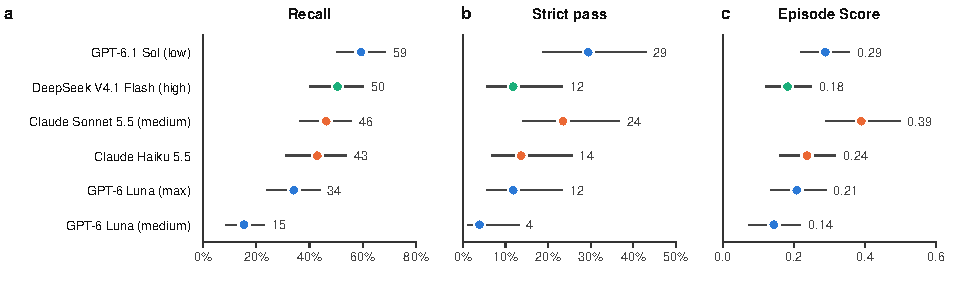
\includegraphics[width=\linewidth]{figures/p2_headline.pdf}
  \caption{\textbf{Headline metrics.} \textbf{a}, Recall; \textbf{b}, strict pass; \textbf{c},
  Episode Score, each with its 95\% interval. Rows are ordered by recall; colour marks the provider.}
  \label{fig:headline}
\end{figure}

Table~\ref{tab:main} and Figure~\ref{fig:headline} give the main results.

\paragraph{No configuration is a reliable release gate.} The best recall is 59\% (Sol) and the best
strict pass rate is 29\%: in about seven of ten releases even the best agent misses a regression or
does not sign off. With false reports forgiven, the best catch credit is 0.66.

\paragraph{Which differences hold.} After correction for multiple comparisons, the differences that
hold separate the strongest configurations from the weakest. On recall, Sol, Sonnet, DeepSeek and
Haiku each exceed Luna medium, Sol exceeds Luna max, and DeepSeek exceeds Luna max. On the Episode
Score, Sonnet exceeds DeepSeek and both Luna configurations, and Sol exceeds Luna medium. On strict
pass only Sol over Luna medium holds. Sol, Sonnet and Haiku are not separated from one another on
any of the three metrics; Sonnet over Haiku on the Episode Score comes closest
($p_\text{Holm} = 0.058$).

\paragraph{The agent that finds most is not the one with the cleanest reports.} Sol catches the
most regressions: paired by episode it leads Sonnet by 15 recall points (95\% interval +2 to +28;
Sol caught more in 17 episodes, Sonnet in 7), though with 15 pairwise comparisons among six
configurations the difference is not significant after correction. Sol also files 164 reports to
Sonnet's 99, and most of the extra reports are false; with precision counted, Sonnet has the higher
Episode Score (0.39 vs 0.29), also not a significant difference. These are differences of profile
rather than established rankings. Figure~\ref{fig:endings}a places each configuration by recall and
precision.

\paragraph{Configurations fail to stop in different ways.} Figure~\ref{fig:endings}b shows how
episodes ended. Sonnet and both Luna configurations sign off in almost every episode, usually with
regressions still present (76--90\% of episodes). DeepSeek is cut off in 82\% of episodes, at the
action cap (78\%) or the report limit (4\%). Haiku stops without signing off in 35\%. No
configuration signs off correctly in more than 29\% of episodes. The confidence reported with a
sign-off does not separate correct from incorrect sign-offs: Sonnet reports about 0.5 and Sol about
0.83 in both cases.

\begin{figure}[!htbp]
  \centering
  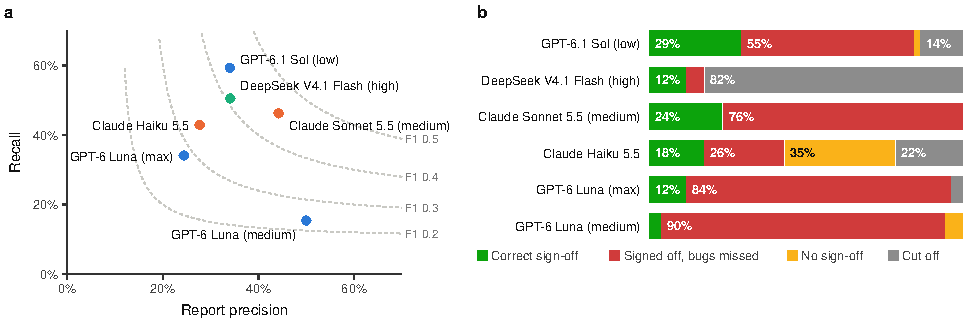
\includegraphics[width=\linewidth]{figures/p3_recall_endings.pdf}
  \caption{\textbf{Finding versus trusting.} \textbf{a}, Recall against report precision; dashed
  lines join points of equal F1. \textbf{b}, How each of the 51 episodes ended.}
  \label{fig:endings}
\end{figure}

\paragraph{More actions do not buy more score.} Sonnet has the highest Episode Score with 67 actions
per episode; Sol, Haiku and DeepSeek use 200--300 and score lower (Figure~\ref{fig:effort}a). By
cost, the frontier runs from Luna medium (\$0.015 per episode) through DeepSeek (\$0.06) and Luna
max (\$0.15) to Sonnet (\$0.54); Sol and Haiku cost more than Sonnet and score less
(Figure~\ref{fig:effort}b).

\paragraph{Effort makes an agent test longer.} Raising GPT-6 Luna from medium to maximum effort
raises recall from 15\% to 34\% (paired permutation test, $p = 0.009$), while precision falls from
0.50 to 0.24 and cost rises about tenfold; the Episode Score rises from 0.14 to 0.21, a difference
that is not significant ($p = 0.24$). Actions per episode rise from 39 to 166, and the changed
features exercised with six or more actions from 27 to 66 of 92. At maximum effort Luna still scores
below Sonnet and Sol at their defaults.

\begin{figure}[!htbp]
  \centering
  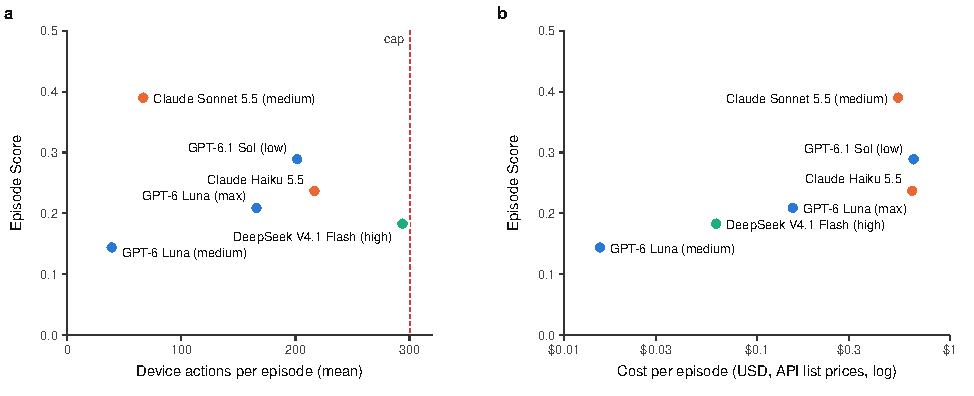
\includegraphics[width=\linewidth]{figures/p4_effort_cost.pdf}
  \caption{\textbf{Effort and cost.} Episode Score against \textbf{a}, mean device actions per
  episode (dashed: the 300-action cap) and \textbf{b}, cost per episode at API list prices (log
  scale).}
  \label{fig:effort}
\end{figure}

\paragraph{\aqb{} and a general index.} For the four configurations with a matching entry, the
Artificial Analysis index and the \aqb{} Episode Score order the configurations almost alike (rank
correlation 0.8); they differ at the top, where the index rates Sol (35) above Sonnet (31) and
\aqb{} ranks Sonnet first on Episode Score and Sol first on recall (Figure~\ref{fig:aa}). The index also reports Sol at low effort spending under
half the time per task of Sonnet at medium; in \aqb{} Sol takes three times as many actions.

\begin{figure}[!htbp]
  \centering
  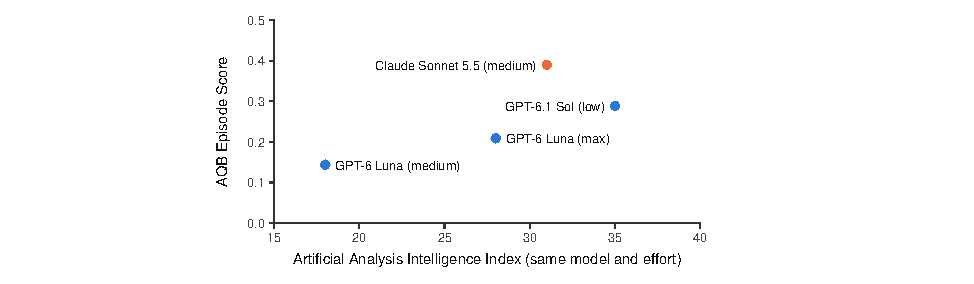
\includegraphics[width=0.85\linewidth]{figures/p6_aa.pdf}
  \caption{\textbf{\aqb{} against a general index.} Episode Score against the Artificial Analysis
  Intelligence Index for the same model and effort.}
  \label{fig:aa}
\end{figure}

% ---------------------------------------------------------------------------
\section{Analysis}\label{sec:analysis}

\subsection{Agents find the changed features but do not break them}
Table~\ref{tab:coverage} and Figure~\ref{fig:coverage} show that every configuration except Luna
medium reaches 78--88 of the 92 changed features, and Sol and DeepSeek reach all but a handful and
ignore none. The misses are in what agents do there: 23--46 regressions per configuration sit in
features the agent exercised with six or more actions and did not break. (A feature counts as on
screen when one of its UI strings appears in an observation; the strings are verified against real
observations for 111 of the 185 release-note lines, and the remaining lines fall back to the
feature's own words.) Sonnet trades depth for
speed: 23 of its 42 catches came from features it looked at for fewer than six actions, more than
any other configuration (10--15), and it also has the most shallow misses among the strong agents
(19).

\begin{table}[!htbp]
\centering\small
\caption{Changelog coverage of the 92 release-note lines that hide a regression.}
\label{tab:coverage}
\begin{tabular}{lrrrrrr}
\toprule
Configuration & Reached & Exercised & Caught & Ignored & Shallow & Not noticed \\
\midrule
GPT-6.1 Sol (low) & 88 & 68 & 54 & 0 & 9 & 29 \\
DeepSeek V4.1 Flash (high) & 87 & 79 & 46 & 0 & 3 & 43 \\
Claude Sonnet 5.5 (medium) & 78 & 44 & 42 & 6 & 19 & 25 \\
Claude Haiku 5.5 & 83 & 72 & 39 & 4 & 6 & 43 \\
GPT-6 Luna (max) & 82 & 66 & 31 & 5 & 10 & 46 \\
GPT-6 Luna (medium) & 68 & 27 & 14 & 20 & 35 & 23 \\
\bottomrule
\end{tabular}
\end{table}

\begin{figure}[!htbp]
  \centering
  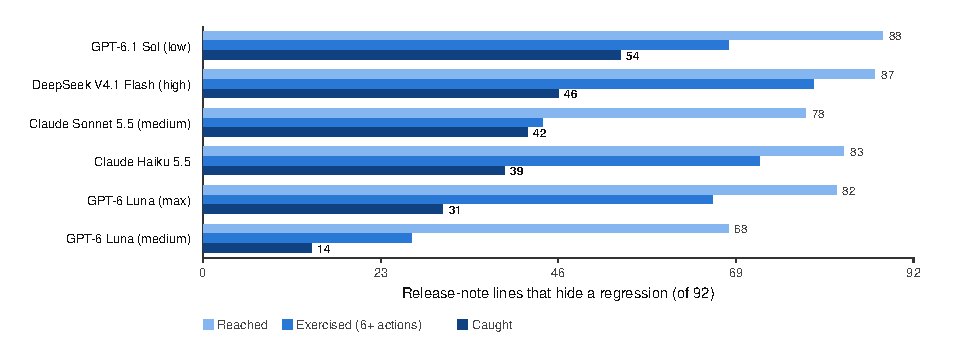
\includegraphics[width=\linewidth]{figures/p5_coverage.pdf}
  \caption{\textbf{Changelog coverage.} Of the 92 release-note lines that hide a regression, how
  many each configuration reached, exercised (six or more actions) and caught.}
  \label{fig:coverage}
\end{figure}

\subsection{Which regressions are caught, and by whom}
Figure~\ref{fig:matrix} shows, for every regression, which configurations caught it. Over all six,
74 of the 91 observable regressions (81\%) are caught at least once and 17 are caught by none. Pairs of configurations
catch more of the same regressions than chance would predict (Sonnet and Sol share 32 catches against
24.5 expected if their catches were independent), yet each also catches regressions the other
misses: 22 only by Sol and 10 only by Sonnet, and DeepSeek catches 6 of the regressions both of them
missed. Many regressions have a narrow trigger, so for these a catch depends on whether the agent
tried one specific action.

\begin{figure}[!htbp]
  \centering
  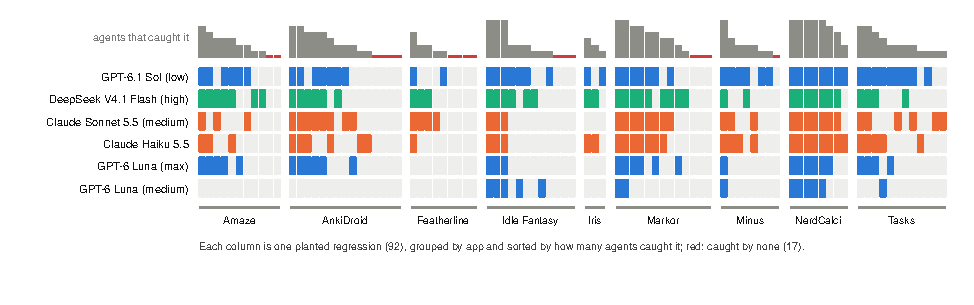
\includegraphics[width=\linewidth]{figures/p8_matrix.pdf}
  \caption{\textbf{Catch matrix.} Each column is one planted regression, grouped by app and sorted
  by how many configurations caught it (bars above); a filled cell means the configuration caught
  it. Red marks the 17 regressions no configuration caught; the one masked regression is not shown.}
  \label{fig:matrix}
\end{figure}

\subsection{The hard core}
The 27 regressions that both Sol and Sonnet missed are not older or newer than the rest (67\% vs
63\% fixed in 2026) and not ported with lower confidence. They fall into four groups:
\begin{itemize}
  \item \textbf{Needs a round trip (6).} A setting must be changed, the file or app closed and
    reopened, and the value checked: an editor's indent size or auto-format, a budget view, the deck
    chosen for new notes, a timebox limit. These are 6 of the 9 ``not persisted'' regressions in
    \aqb{}.
  \item \textbf{Needs a specific input or action (10).} Long-pressing \emph{Bold} (which closes the
    app), choosing \emph{Select all} twice, typing seven digits into a five-digit field, saving an
    empty weight, renaming ``French'' to ``FRENCH'', or duplicating a last line with no trailing
    newline. Sol and DeepSeek spent 133 and 151 actions with the formatting toolbar on
    screen without long-pressing \emph{Bold}.
  \item \textbf{Needs to know what is correct (10).} The screen looks plausible
    (Figure~\ref{fig:hard}): 2,567,890 coins shown as 2.6M where the format floors to 2.5M, a Videos
    filter that says ``No photos found'', a start-date chip that repeats the due date, ``04:00''
    among times written in AM/PM, farm produce listed as junk to sell, or sort options shown for a
    scheduler that is off.
  \item \textbf{Multi-step state (1).} A favourite star out of sync after a dialog.
\end{itemize}
The first two groups correspond directly to instructions in the prompt (``after a change, leave and
come back, and check that it was kept''; ``repeat an action''; ``try empty, boundary and unusual
values''), and the prompt states that signing off with regressions unreported is the worst outcome.
Agents apply the generic checks but rarely the targeted ones (Table~\ref{tab:actions}). Sol, Haiku
and Luna max rotate the device in every episode, yet Sol long-presses in only 7 of 51 episodes, and
Sonnet re-opens the app in 13. In the episodes where Sonnet missed a regression it signed off after
about 70 of its 300 available actions. The misses therefore lie in carrying out the stated method
over a long, open-ended session: the method is in every prompt.

\begin{table}[!htbp]
\centering\small
\caption{Episodes (of 51) in which each configuration used an action the QA method calls for.
Re-opening counts \texttt{open\_app} only; re-opening a file inside the app is not counted.}
\label{tab:actions}
\begin{tabular}{lrrrr}
\toprule
Configuration & Rotate & Re-open app & Long-press & Type text \\
\midrule
GPT-6.1 Sol (low) & 51 & 27 & 7 & 51 \\
DeepSeek V4.1 Flash (high) & 49 & 29 & 36 & 48 \\
Claude Sonnet 5.5 (medium) & 23 & 13 & 16 & 34 \\
Claude Haiku 5.5 & 51 & 29 & 21 & 40 \\
GPT-6 Luna (max) & 51 & 14 & 30 & 46 \\
GPT-6 Luna (medium) & 44 & 6 & 15 & 23 \\
\bottomrule
\end{tabular}
\end{table}

\begin{figure}[!htbp]
  \centering
  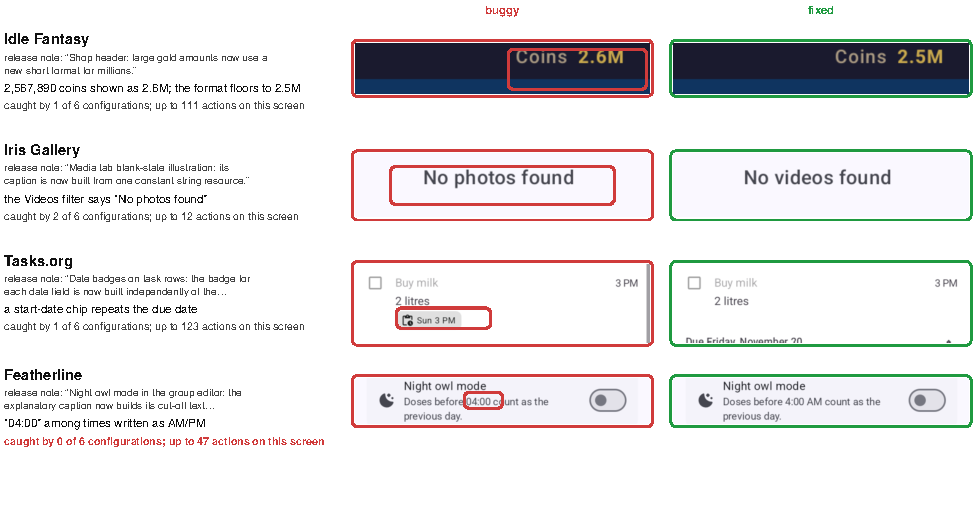
\includegraphics[width=\linewidth]{figures/p7_hard.pdf}
  \caption{\textbf{Regressions both Sol and Sonnet missed}, as the device shows them on the buggy and
  fixed builds (calibration screenshots; the defect circled). Each row gives the release-note line
  the agent received, how many of the six configurations caught the regression, and the most
  actions any configuration spent with that screen on display.}
  \label{fig:hard}
\end{figure}

\subsection{Contamination}
If agents had memorised upstream fixes, older regressions would be easier. There is no consistent
difference: Sol catches 19 of 33 regressions fixed before 2026 and 35 of 58 fixed in 2026, Sonnet
17/33 and 25/58, DeepSeek 16/33 and 30/58. Agents have no network or file access during an episode.

% ---------------------------------------------------------------------------
\section{Discussion}

\paragraph{Distance from saturation.} The best single configuration reaches 59\% recall, 29\% strict
pass and an Episode Score of 0.39, and a per-regression oracle over all six configurations still
misses 19\% of the observable regressions. Because real but unplanted app behaviour counts as false reports,
the Episode Score of a perfect agent can fall slightly below 1; recall and strict pass have no such
ceiling.

\paragraph{Which metric for which gate.} For a release gate that a person reviews, a missed regression
costs more than a false report, and recall ranks the configurations; there Sol leads. For a gate
whose reports go to developers directly, precision and correct sign-off matter, and the Episode Score
ranks them; there Sonnet leads.

% ---------------------------------------------------------------------------
\section{Limitations}
\begin{itemize}
  \item \textbf{One run per episode.} Intervals are wide, configurations in the middle of the ranking
    (Haiku, Luna max, DeepSeek) are not separated by score, and part of the difference in which
    regressions each configuration caught is run-to-run variance.
  \item \textbf{Harness and model are confounded.} Each model ran in its vendor's harness at its
    default effort.
  \item \textbf{Configurations.} The largest models (e.g.\ Claude Opus 5.5) and maximum effort for
    every model were not evaluated.
  \item \textbf{Release notes.} The notes were written by the authors in real changelog style; some
    lines are more specific than others.
  \item \textbf{Grading.} The matcher credits 84\% of correct reports in its blind audit, so a missed
    credit can be the grader's. Every rejected report of the first two full runs was checked by hand;
    later runs were not.
  \item \textbf{Calibration.} Each check was verified once on a device; two regressions depend on
    environment details (the order of equal sort keys, the device's 12-hour clock).
  \item \textbf{Scale.} 9 apps, 51 episodes and 92 regressions.
\end{itemize}

% ---------------------------------------------------------------------------
\section{Conclusion}
\aqb{} asks LLM agents to do release QA on real Android apps with planted, device-verified
regressions and deterministic grading. Current agents reach the changed features but catch at most
59\% of the regressions, sign off correctly in at most 29\% of releases, and 19\% of the regressions
escape every configuration. The misses concentrate in verification steps the agents were told to
use: re-opening after a change, trying the specific input, and checking values against what they
should be.

\bibliographystyle{plainnat}
\bibliography{refs}

% ---------------------------------------------------------------------------
\appendix
\section{Example brief}\label{app:brief}
The brief of episode \texttt{tasks-E05} (two planted regressions: the second and fourth changelog
lines):
\begin{quote}\small
\textbf{QA sweep: Tasks.org.} The app is installed and open. A colleague asked you to sweep these
areas before release: sorting and grouping options; task notes and links.\\[2pt]
\textbf{Preconditions.} The list contains: Buy milk (due in 5 days, notes `2 litres'); Pack for
trip (due in 10 days) with subtasks Charge phone and Print tickets; Pay rent (due in 20 days)
repeating monthly; and Read docs (no due date), whose notes contain the link
https://example.com/guide.\\[2pt]
\textbf{Changed in this build.}
\begin{itemize}
  \item Link handling in task notes: web links are now detected when the note is displayed.
  \item Name-based sorting: tasks are now sorted by a key produced by a shared helper.
  \item Due date grouping in the task list: group headings are now generated from the user's date
    format.
  \item Subtasks section of the sort sheet: its controls are now built the same way for every option.
\end{itemize}
\end{quote}

\section{QA method given to every agent}\label{app:method}
\begin{quote}\small
How to test well (general QA practice):
\begin{itemize}
  \item Make a plan from the areas above and exercise every one of them before you sign off.
    Signing off while bugs remain unreported is the worst outcome, worse than spending more steps.
  \item Go past the happy path. For each feature, also check:
  \begin{itemize}
    \item State: after a change, leave and come back, and check that it was kept.
    \item Reversal: undo, cancel or reverse a change, and check the app returns to the right state.
    \item Repetition: repeat an action, and check the result is still right.
    \item Input: try empty, boundary and unusual values.
    \item Consistency: check that what each screen shows agrees with the data, and with other screens.
    \item Device: rotate the screen, and check that nothing is lost.
    \item Navigation: reach screens by more than one route.
  \end{itemize}
  \item Use the starting data described in the preconditions in your tests.
  \item Reproduce a problem once before you report it.
\end{itemize}
\end{quote}

\section{Pairwise differences}\label{app:pairwise}
Per-episode mean difference (first minus second configuration) and Holm-corrected $p$ from a paired
sign-flip permutation test over the 51 episodes, for each of the 15 pairs. Strict pass is in
\texttt{docs/RESULTS.md}.
\begin{table}[h]
\centering\small
\begin{tabular}{lrrrr}
\toprule
Pair & Recall diff & $p_\text{Holm}$ & Episode Score diff & $p_\text{Holm}$ \\
\midrule
Sonnet vs Luna medium & +0.288 & $<$0.001 & +0.246 & 0.006 \\
Sol vs Luna max & +0.294 & $<$0.001 & +0.081 & 0.674 \\
Sol vs Luna medium & +0.441 & $<$0.001 & +0.145 & 0.026 \\
DeepSeek vs Luna medium & +0.327 & $<$0.001 & +0.039 & 1.000 \\
Haiku vs Luna medium & +0.278 & 0.001 & +0.093 & 0.656 \\
Luna max vs DeepSeek & -0.180 & 0.011 & +0.026 & 1.000 \\
Sol vs Haiku & +0.163 & 0.057 & +0.052 & 1.000 \\
Sonnet vs Luna max & +0.141 & 0.061 & +0.181 & 0.004 \\
Luna max vs Luna medium & +0.147 & 0.065 & +0.064 & 1.000 \\
Haiku vs Luna max & +0.131 & 0.165 & +0.029 & 1.000 \\
Sonnet vs Sol & -0.154 & 0.165 & +0.100 & 0.656 \\
Sol vs DeepSeek & +0.114 & 0.433 & +0.107 & 0.237 \\
Haiku vs DeepSeek & -0.049 & 1.000 & +0.054 & 0.848 \\
Sonnet vs DeepSeek & -0.039 & 1.000 & +0.207 & $<$0.001 \\
Sonnet vs Haiku & +0.010 & 1.000 & +0.153 & 0.058 \\
\bottomrule
\end{tabular}

\end{table}

\section{Recall by app}
\begin{table}[h]
\centering\small
\begin{tabular}{lrrrrrr}
\toprule
App & Sol & DeepSeek & Sonnet & Haiku & Luna max & Luna med \\
\midrule
Amaze (11) & 6 & 7 & 3 & 3 & 5 & 0 \\
AnkiDroid (15) & 7 & 6 & 8 & 6 & 6 & 0 \\
Featherline (9) & 2 & 3 & 4 & 1 & 0 & 0 \\
Idle Fantasy (12) & 7 & 6 & 3 & 3 & 3 & 5 \\
Iris (3) & 2 & 2 & 0 & 2 & 0 & 0 \\
Markor (13) & 7 & 9 & 8 & 7 & 6 & 2 \\
Minus (8) & 6 & 2 & 3 & 4 & 1 & 1 \\
NerdCalci (8) & 8 & 7 & 7 & 8 & 6 & 5 \\
Tasks (12) & 8 & 4 & 6 & 5 & 4 & 1 \\
\bottomrule
\end{tabular}
\end{table}

\end{document}
